\section{Introduction}\label{s:intro}
There is a growing desire to perform more complex analyses on the increasing amounts of data being gathered. 
This data is connected, which will often be represented and thought of as a  graph~\cite{DBLP:journals/debu/ShaoLWX17}.  
An extended survey of Sahu et al.~\cite{DBLP:journals/vldb/SahuMSLO20} shows that graphs are used across a very diverse range of domains. 
Graphs often provide a natural way to structure data involving entities, represented as vertices, and the relationships between them, represented as edges.
In turn, this increased desire has caused an increased rise in the attention given to graph database management systems (GDBMSs)~\cite{Fan2015TheCA}.
These systems provide a new way of visualising and analysing graph data.
However, the performance of these systems often leaves to be desired~\cite{DBLP:journals/pvldb/Ozsu19, Fan2015TheCA}. 
The question is whether there is a need for this new method of looking at the data.
Traditional relational database management systems (RDBMSs) are perfectly capable of storing graph data by using a vertex table and an edge table. 
Still, providing a way to perform these more complex analyses has been difficult up to now due to the limitations of the standard query language SQL~\cite{oracle-sql-example}.

In response to the limited capabilities, a plethora of GDBMSs arose, each having its own graph query language~\cite{DBLP:journals/corr/abs-1910-09017}.
Examples of systems and their query languages are TigerGraph with GSQL~\cite{tigergraph}, Neo4j with Cypher~\cite{Francis2018}, Oracle Labs PGX with Property Graph Query Language (PGQL)~\cite{10.1145/2960414.2960421}. Amazon Neptune even supports three distinct languages, namely OpenCypher, Gremlin, and SPARQL. 
Within these graph query languages, it is often easier to write queries containing graph pattern matching and path finding. 
However, each query language has a different syntax, different semantics, and different capabilities. 
These problems make working with graph-based data cumbersome for users.

The limited capabilities of SQL will change, as an extension of SQL is scheduled to release in March of 2023 called SQL/Property Graph Query (SQL/PGQ), making it easier to support this new type of workload related to graph data in RDBMSs~\cite{isosqlpgq}.

For querying graph data, two functionalities are deemed most important: \textit{graph pattern matching} and \textit{path finding}~\cite{DBLP:journals/csur/AnglesABHRV17}.
In SQL it is possible to write queries containing graph pattern matching and path finding, but, these queries are often hard to write, understand, and inefficient to evaluate~\cite{graindb}. 
In particular, path finding requires using recursive queries. 
An example can be found in Listing~\ref{app:sqlquery1}, which shows a path finding query that returns all paths starting from \textit{Person 1}~\cite{DuckDBDocumentationWithClause}. 
Support for this was added in SQL:1999~\cite{Melton2002Sql1U}, and is supported by popular RDBMSs such as PostgreSQL and SQLite.
However, as shown by Michels and Witkowski~\cite{oracle-sql-example}, even relatively simple graph queries in plain SQL take up many lines and are more difficult to understand compared to the equivalent query in SQL/PGQ. 
The goal of SQL/PGQ is to provide a more compact syntax for graph-like data and make path finding queries, such as reachability or shortest path, more accessible.

% The amount of highly interconnected data is growing at an unprecedented pace~\cite{DBLP:journals/cacm/SakrBVIAAAABBDV21}, making the ability to accurately and effectively process and analyze graph-based data more difficult. 
% A survey conducted by Hegeman and Iosup~\cite{DBLP:journals/corr/abs-1807-00382} in 2018 showed that there is a large diversity in the domains that contain graph features and make use of graph analysis methods, including biology, security, logistics \& planning, sociology, and finance. 
% However, the increasing popularity revealed that for many use cases Relational Database Management Systems (RDBMSs) were running into performance issues due to the structure of the data being highly interconnected~\cite{DBLP:journals/cacm/SakrBVIAAAABBDV21, DBLP:journals/debu/ShaoLWX17}.

Work on a standardization of a graph query language started in 2018~\cite{DBLP:conf/sigmod/AnglesABBFGLPPS18, Deutsch2021, gqlmanifesto}. 
Currently the \emph{ISO/IEC JTC1 SC32 WG3 Database Languages} working group is developing SQL/PGQ, which will become part of the upcoming SQL:2023 standard~\cite{isosqlpgq}. 
In SQL/PGQ a graph can be defined in terms of tables~\cite{DBLP:conf/sigmod/MhedhbiLKWS21} and queries can contain special syntax for path finding and graph pattern matching.
The standard is limited to read-only queries, as it will not be possible to modify the graph through the graph tables in SQL/PGQ. 
Therefore, the same workgroup is also working on Graph Query Language (GQL)~\cite{isogql}, in which it will be possible to modify the data in addition to all the features contained in SQL/PGQ.
GQL will be a superset in relation to SQL/PGQ, see Figure~\ref{fig:sqlpgqgql}, which will have the ability to manipulate the data.

\begin{figure}
  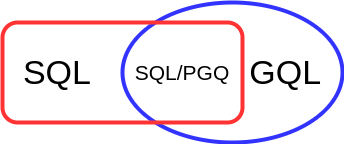
\includegraphics[width=0.5\linewidth]{figures/SQLPGQ-GQL.png}
  \caption{SQL/PGQ in relation to SQL and GQL.}
  \label{fig:sqlpgqgql}
\end{figure}

% Additionally, the standardised query language used in RDBMSs, SQL, will be releasing an extension called SQL/Property Graph Query (SQL/PGQ) in September 2022~\cite{Deutsch2021}. 
% This extension will make it easier to write queries with \textit{graph patterns} and navigational expressions in SQL.

In this thesis we integrate the SQL/PGQ standard in DuckDB.
DuckDB is an open-source in-process SQL OLAP database management system produced~\cite{DBLP:conf/sigmod/RaasveldtM19} by CWI~\cite{duckdblabs}. 
With the new SQL/PGQ standard releasing soon, work on integrating it into DuckDB has already started by Singh et al.~\cite{sqlpgq-duckdb}. 
However, the standard has not been fully integrated as of now. In particular the shortest and cheapest path functions are not yet implemented. Additionally, the feature to return the nodes contained in these cheapest and shortest path functions will also be implemented.
Therefore, the goal is to complete this integration by adding these functionalities. Additionally, we will identify and implement various optimizations especially related to typical graph queries in DuckDB.
% In the current state SQL/PGQ queries can be parsed and the reachability of a node, given a source node, can be computed. 
% The next step is to compute the path length and eventually be able to retrieve the path. 
% Essentially being able to compute various numbers of graph traversal operations. 

The structure of this thesis proposal is as follows. Section~\ref{sec:background} discusses relevant background information regarding graphs and SQL/PGQ. In Section~\ref{sec:goals} we formulate the research questions and the goals of this thesis. Section~\ref{sec:method} describes how the research questions will be answered and evaluated and provides a research plan. We end with a conclusion in Section~\ref{sec:conclusion}.  






% \subsection{Why is it interesting and important?}

% \subsection{Why is it hard? (E.g., why do naive approaches fail?)}

% \subsection{Why hasn't it been solved before? (Or, what's wrong with previous proposed solutions? How does mine differ?)}
% \subsection{What are the key components of my approach and results? Also include any specific limitations.}














% Graph databases have seen an increase in popularity in the last few years. 
% Graphs provide an intuitive way of storing and visualizing data, an example of this is Wikidata which stores its data in the form of open-source knowledge graphs~\cite{10.1145/2629489}. This data is provided in the Resource Description Framework (RDF) format, which is a form of direct edge-labelled graphs. Another way of storing data is by using the property graph data model, which is a form of a mixed multigraph model. In these models both nodes and edges can have labels, as well as properties, a more detailed description will be provided in Section~\ref{sec:background}. 

% Working with property graph data models in SQL is possible, however cumbersome and graph-based queries can be difficult to write and understand~\cite{graindb}. 
% Only recently has there been a proposal for the SQL standard to be expanded upon with the addition of the Graph Query Language (GQL)~\cite{gqlproposal}. 
% Initiative was taken in 2018 with the GQL manifesto~\cite{gqlmanifesto} by A. Green. 
% At the time, many separate graph query languages existed. However, three languages were chosen as the inspiration for GQL, namely Cypher originally created by Neo4j and currently maintained by OpenCypher, Property Graph Query Language (PGQL) by Oracle and G-CORE, a research language from the Linked Database Benchmarking Council (LDBC). 
% The proposal for GQL was accepted by the JTC1-the committee in joint charge of information technology standard for the International Organization for Standardization (ISO), and International Electrotechnical Commission (IEC)~\cite{Deutsch2021} and as such, the SQL standard will be extended with SQL/Property Graph Query (SQL/PGQ). SQL/PGQ specifies how graph views should be defined over an SQL tabular schema, and running read-only queries against them.  

% The main topic of this thesis is to integrate the SQL/PGQ standard as defined in DuckDB. DuckDB is an open-source in-process SQL OLAP database managament system produced by DuckDB labs, a spin-off company at CWI~\cite{duckdblabs}. With the new SQL/PGQ standard recently having been approved, work on integrating it into DuckDB has already started by Singh et al.~\cite{sqlpgq-duckdb}. However, the standard has not been fully integrated as of now. In the current state SQL/PGQ queries can be parsed and the reachability of a node, given a source node, can be computed. The next step is to compute the path length, and eventually be able to retrieve the path. Essentially being able to compute various numbers of graph traversal operations. 

% In addition, the performance of DuckDB can be further optimized in certain cases. In particular, when a query is executed containing a join operation on the same table ($Table A \Join Table A$), two hash tables are built for each table. However, these hash tables are equal and therefore only a single one would suffice, reducing memory usage and saving time on building the hash table. This case occurs often when querying graph tables in RDBMSs, since the graphs are stored in two tables, the vertex table (containing a $node_id$) and the edge table (containing a $source_node_id$ and a $destination_source_id$). Whenever a query is performed on these tables, we join the vertex table twice on the edge table (once on the $source_node_id$ and once on the $destination_node_id$). 

% In spirit, this thesis contains similarities to the work performed by Jin et al.~\cite{graindb}. They created GRainDB, a system which extended DuckDB with graph modeling, querying, and visualization capabilities. However, they based their query language GRQL from TigerGraph's GSQL~\cite{tigergraph} and Oracle's PGQL~\cite{10.1145/2960414.2960421}. Thus, this thesis differs in that the goal will be to integrate the standardized SQL/PGQ. 

% The structure of this thesis proposal is as follows. Section~\ref{sec:background} will discuss relevant background information regarding graphs and SQL/PGQ. In Section~\ref{sec:goals} we formulate the research questions and the goals of this thesis proposal. Section~\ref{sec:method} will describe how the research questions will be answered and evaluated and provides a small concrete planning. We end with a conclusion in Section~\ref{sec:conclusion}.  

% \subsection{Why would SQL/PGQ be better}





